%%##################################################
\frame{
\frametitle{Hochschulkommunikation}
	\begin{block}{Kommunikation mit Hochschul-Content}
		\begin{itemize}
			\item Hochschule interne Daten �ber Content System
			\item Content-Zugriff bei Internetzugriff des Mobilfunktger�ts
		\end{itemize}
		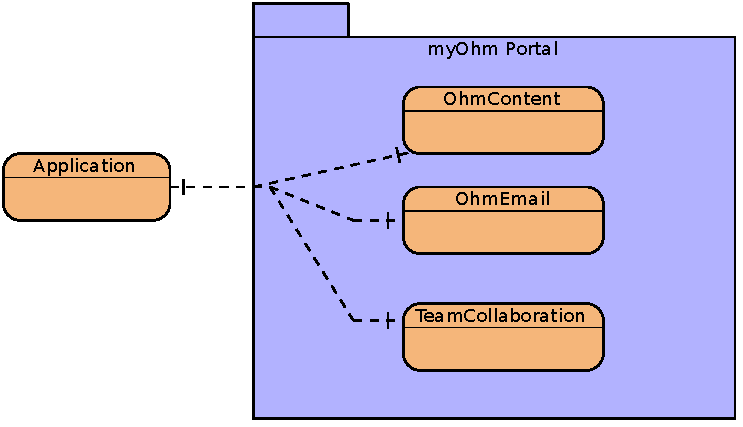
\includegraphics[width=0.7\textwidth]{../grafiken/OhmCollab.pdf}
	\end{block}
}

\frame{
\frametitle{Datenhaltung}
	\begin{block} {Content Management System (CMS)}
	\begin{itemize}
		\item CMS zum Verwalten von Inhalten
		\item Verschiedene Benutzerrollen:	
			\begin{itemize}
				\item Administrator: Bearbeitung von Design und Inhalt
				\item Redakteuer: Bearbeitung von Inhalt
			\end{itemize}
		\item $\rightarrow$ Hochschule benutzt bereits CMS Systeme f�r Inhalte der Webseite. \\\textbf{Vorteil: zus�tzliche Schulung nicht notwendig} 
	\end{itemize}
	\end{block}
	\begin{block} {Datenbank}
	\begin{itemize}
		\item mySQL-Datenbank	
		\item zyklisches Aktualisieren auf Endanwendung
	\end{itemize}
	\end{block}
}

\frame{
\frametitle{Zusammenspiel}
	\begin{block}{Diagramm}
		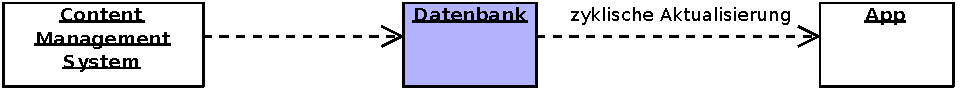
\includegraphics[width=1.0\textwidth]{../grafiken/DB.pdf}
	\end{block}
}
